% Options for packages loaded elsewhere
\PassOptionsToPackage{unicode}{hyperref}
\PassOptionsToPackage{hyphens}{url}
%
\documentclass[
]{book}
\usepackage{lmodern}
\usepackage{amssymb,amsmath}
\usepackage{ifxetex,ifluatex}
\ifnum 0\ifxetex 1\fi\ifluatex 1\fi=0 % if pdftex
  \usepackage[T1]{fontenc}
  \usepackage[utf8]{inputenc}
  \usepackage{textcomp} % provide euro and other symbols
\else % if luatex or xetex
  \usepackage{unicode-math}
  \defaultfontfeatures{Scale=MatchLowercase}
  \defaultfontfeatures[\rmfamily]{Ligatures=TeX,Scale=1}
\fi
% Use upquote if available, for straight quotes in verbatim environments
\IfFileExists{upquote.sty}{\usepackage{upquote}}{}
\IfFileExists{microtype.sty}{% use microtype if available
  \usepackage[]{microtype}
  \UseMicrotypeSet[protrusion]{basicmath} % disable protrusion for tt fonts
}{}
\makeatletter
\@ifundefined{KOMAClassName}{% if non-KOMA class
  \IfFileExists{parskip.sty}{%
    \usepackage{parskip}
  }{% else
    \setlength{\parindent}{0pt}
    \setlength{\parskip}{6pt plus 2pt minus 1pt}}
}{% if KOMA class
  \KOMAoptions{parskip=half}}
\makeatother
\usepackage{xcolor}
\IfFileExists{xurl.sty}{\usepackage{xurl}}{} % add URL line breaks if available
\IfFileExists{bookmark.sty}{\usepackage{bookmark}}{\usepackage{hyperref}}
\hypersetup{
  pdftitle={Fundamentos de Inferência Bayesiana},
  pdfauthor={Victor Fossaluza},
  hidelinks,
  pdfcreator={LaTeX via pandoc}}
\urlstyle{same} % disable monospaced font for URLs
\usepackage{longtable,booktabs}
% Correct order of tables after \paragraph or \subparagraph
\usepackage{etoolbox}
\makeatletter
\patchcmd\longtable{\par}{\if@noskipsec\mbox{}\fi\par}{}{}
\makeatother
% Allow footnotes in longtable head/foot
\IfFileExists{footnotehyper.sty}{\usepackage{footnotehyper}}{\usepackage{footnote}}
\makesavenoteenv{longtable}
\usepackage{graphicx,grffile}
\makeatletter
\def\maxwidth{\ifdim\Gin@nat@width>\linewidth\linewidth\else\Gin@nat@width\fi}
\def\maxheight{\ifdim\Gin@nat@height>\textheight\textheight\else\Gin@nat@height\fi}
\makeatother
% Scale images if necessary, so that they will not overflow the page
% margins by default, and it is still possible to overwrite the defaults
% using explicit options in \includegraphics[width, height, ...]{}
\setkeys{Gin}{width=\maxwidth,height=\maxheight,keepaspectratio}
% Set default figure placement to htbp
\makeatletter
\def\fps@figure{htbp}
\makeatother
\setlength{\emergencystretch}{3em} % prevent overfull lines
\providecommand{\tightlist}{%
  \setlength{\itemsep}{0pt}\setlength{\parskip}{0pt}}
\setcounter{secnumdepth}{5}
\usepackage{booktabs}
\usepackage[]{natbib}
\bibliographystyle{apalike}

\title{Fundamentos de Inferência Bayesiana}
\author{Victor Fossaluza}
\date{2020-05-14}

\begin{document}
\maketitle

{
\setcounter{tocdepth}{1}
\tableofcontents
}
Essas notas de aula tem o intuito apenas de ser um guia de estudos e não necessariamente irá apresentar todo o conteúdo da disciplina de \emph{Inferência Bayesiana}. Além disso, esta é uma versão preliminar e está bem longe de ser uma versão final, de modo que podem haver muitos erros e correções ou sugestões seráo bem vindas!

\hypertarget{ProbSubj}{%
\chapter{PROBABILIDADE SUBJETIVA}\label{ProbSubj}}

A construção de probabilidade subjetiva apresentada aqui pode ser encontrada em \citet{DeGroot70}.

\hypertarget{aula-01}{%
\section{Aula 01}\label{aula-01}}

\begin{itemize}
\tightlist
\item
  \(\Omega\): \emph{espaço amostral}, conjunto não vazio.
\end{itemize}

\(~\)

\begin{itemize}
\tightlist
\item
  \(\mathcal{A}\): \emph{\(\sigma\)-álgebra de subconjuntos} de \(\Omega\), isto é,

  \begin{enumerate}
  \def\labelenumi{\arabic{enumi}.}
  \tightlist
  \item
    \(\Theta \in \mathcal{A}\);
  \item
    \(A \in \mathcal{A} \Longrightarrow A^{c} \in \mathcal{A}\);
  \item
    \(\displaystyle A_1, A_2, \ldots \in \mathcal{A} \Longrightarrow \bigcup_{i\geq1} A_i \in \mathcal{A}\).
  \end{enumerate}
\item
  Os elementos de \(\mathcal{A}\) são chamados de \emph{eventos} e serão denotados por \(A, B, C, \ldots, A_1, A_2, \ldots\)
\end{itemize}

\hypertarget{definiuxe7uxe3o-axiomuxe1tica}{%
\subsection{Definição Axiomática}\label{definiuxe7uxe3o-axiomuxe1tica}}

\begin{itemize}
\tightlist
\item
  \(P: \mathcal{A} \longrightarrow [0,1]\) é uma \emph{medida de probabilidade} se

  \begin{enumerate}
  \def\labelenumi{\arabic{enumi}.}
  \tightlist
  \item
    \(P(\Omega) = 1\);
  \item
    \(\displaystyle A_1, A_2, \ldots \in \mathcal{A}\) com \(A_i \bigcap A_j = \emptyset\) , \(\displaystyle P\left(\bigcup_{i \geq 1} A_i\right) = \sum_{i \geq 1} P\left(A_i\right)\).
  \end{enumerate}
\end{itemize}

\hypertarget{interpretauxe7uxf5es-de-probabilidade}{%
\subsection{Interpretações de Probabilidade}\label{interpretauxe7uxf5es-de-probabilidade}}

\begin{itemize}
\tightlist
\item
  \textbf{Interpretação Clássica} (De Moivre, Laplace)

  \begin{itemize}
  \tightlist
  \item
    baseia-se na equiprobabilidade dos resultados;
  \item
    \(P(A) = \frac{|A|}{|\Omega|}\).
  \item
    \textbf{Exemplo:} um lançamento de moeda, \(A\) = ``cara'', \(P(A) = \frac{1}{2}\).
  \end{itemize}
\end{itemize}

\(~\)

\begin{itemize}
\tightlist
\item
  \textbf{Interpretação Frequentista} (Venn, von Mises, Reichenbach, etc.)

  \begin{itemize}
  \tightlist
  \item
    quase unânime na primeira metade do século XX e ainda é a mais aceita;
  \item
    baseia-se na regularidade das frequências relativas (lei dos grandes números);
  \item
    \(P(A) = lim \frac{A_n}{n}\), onde \(A_n\) é o número de ocorrências de \(A\) em \(n\) realizações \emph{idênticas e independentes} do experimento;
  \item
    Supõe que é possível repetir indefinidamente o experimento nas mesmas circustâncias.
  \item
    \textbf{Exemplo:} um lançamento de moeda, \(A\) = ``cara''.
  \end{itemize}
\end{itemize}

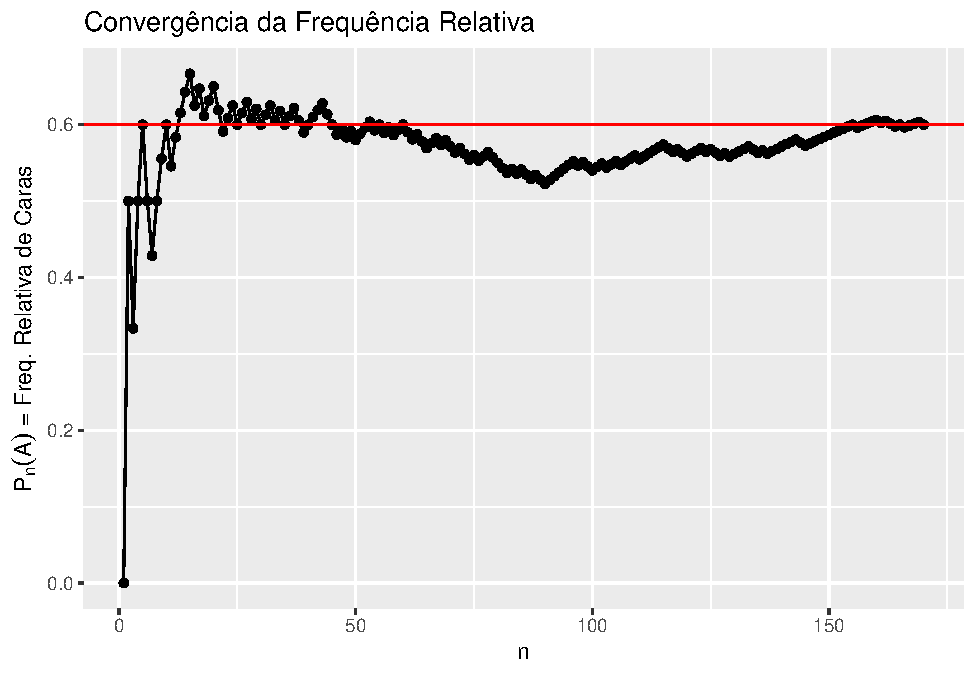
\includegraphics{InfBayes_files/figure-latex/unnamed-chunk-1-1.pdf}

\(~\)

\begin{itemize}
\tightlist
\item
  \textbf{Interpretação Lógica} (Keynes, Jeffreys, Carnap, etc.)

  \begin{itemize}
  \tightlist
  \item
    medida de ``vínculo parcial'' entre uma evidência e uma hipótese;
  \item
    baseia-se em relações objetivas entre proposições.
  \item
    \textbf{Exemplo:} considere duas proposições: ``até agora todos os lançamentos resultaram em cara'' e ``será realizado um novo lançamento''. Pode-se afirmar que ``provavelmente o resultado do novo lançamento será cara''.
  \end{itemize}
\end{itemize}

\(~\)

\begin{itemize}
\tightlist
\item
  \textbf{Interpretação Subjetivista} (Ramsey, de Finetti, Savage, etc)

  \begin{itemize}
  \tightlist
  \item
    probabilidade como medida subjetiva de crença;
  \item
    baseada na experiência de cada indivíduo, portanto única.
  \item
    \textbf{Exemplo:} suponha que Bruno lançou uma moeda 3 vezes e todos os resultados foram cara. Esse indivíduo, em posse dessa informação, pode acreditar que o resultado cara é mais provável que coroa. Contudo, quando pergunta sobre a probabilidade de cara ao seu colega Olavo, ignorante com relação a moeda, ele responde que é 1/2.
  \end{itemize}
\end{itemize}

\(~\)

\hypertarget{aula-02}{%
\section{Aula 02}\label{aula-02}}

\hypertarget{relauxe7uxe3o-de-crenuxe7a-precsim}{%
\subsection{\texorpdfstring{Relação de Crença \(\precsim\)}{Relação de Crença \textbackslash precsim}}\label{relauxe7uxe3o-de-crenuxe7a-precsim}}

\(\precsim\) : relação de ``crença'' em \(\mathcal{A}\times\mathcal{A}\)

\begin{itemize}
\tightlist
\item
  \(A \prec B\) : acredito mais em \(B\) que em \(A\) (\(B \succ A\))
\item
  \(A \sim B\) : acredito igualmente em \(B\) e \(A\)
\item
  \(A \precsim B\) : acredito em \(B\) pelo menos tanto quanto em \(A\)
\end{itemize}

\textbf{Objetivo:} sob certas condições em \(\precsim\), obter uma medida de probabilidade \(P\) que representa (concorda) com \(\precsim\).

\[A \precsim B ~ \Longleftrightarrow ~ P(A) \leq P(B)\]

\hypertarget{suposiuxe7uxf5es-sobre-precsim}{%
\subsection{\texorpdfstring{Suposições sobre \(\precsim\)}{Suposições sobre \textbackslash precsim}}\label{suposiuxe7uxf5es-sobre-precsim}}

\begin{quote}
\textbf{SP1:} Para \(A, B \in \mathcal{A}\), exatamente uma das afirmações a seguir deve valer:\\
\[A \prec B ~,~ B \prec A ~\textrm{ou}~ A \sim B.\]
\end{quote}

\(~\)

\begin{quote}
\textbf{SP2:} \(A_1, A_2, B_1, B_2 \in \mathcal{A}\) tais que \(A_1 \cap A_2 = B_1 \cap B_2 = \emptyset\) e \(A_i \precsim B_i\), \(i=1,2\). Então
\[A_1 \cup A_2 \precsim B_1 \cup B_2 .\]
Além disso, se \(A_i \prec B_i\) para algum \(i\), então \(A_1 \cup A_2 \prec B_1 \cup B_2 .\)
\end{quote}

\(~\)

\begin{quote}
\textbf{SP3:} Se \(A\) é um evento, então \(\emptyset \precsim A\). Além disso, \(\emptyset \prec \Omega\).
\end{quote}

\(~\)

\begin{quote}
\textbf{SP4:} Se \(A_1, A_2, \ldots\) uma sequência decrescente de eventos, isto é, \(A_n \supseteq A_{n+1}, \forall n\), e \(B\) tal que \(B \precsim A_n, \forall n\) então \[B \precsim \bigcap_{n \geq 1} A_n.\]
\end{quote}

\(~\)

\begin{quote}
\textbf{SP5:} Existe uma variável aleatória \(X: \Omega \longrightarrow \mathbb{R}\), \(\mathcal{A}\)-mensurável, tal que \(X(\omega) \in [0,1], \forall \omega \in \Omega\) e, se \(I_1\) e \(I_2\) são intervalos contidos em \([0,1]\), \(\{X \in I_1\} \precsim \{X \in I_2\} \Leftrightarrow \lambda(I_1) \leq \lambda(I_2)~.\)
\end{quote}

\begin{itemize}
\item
  Se \(I=[a,b] \subseteq [0,1]\), \(\lambda(I) = b-a\) é o comprimento do intervalo \(I\) (medida de Lebesgue).
\item
  ``Experimento auxiliar'' ; \(X \sim\) Uniforme{[}0,1{]}.
\item
  \(\{X \in [a,b]\}\) \(\sim \{X \in (a,b]\}\) \(\sim \{X \in [a,b)\}\) \(\sim \{X \in (a,b)\}\).
\end{itemize}

\(~\)

\textbf{Lema 1:} \(A, B, D \in \mathcal{A}\) tais que \(A \cap D = B \cap D = \emptyset\). Então \[A \precsim B ~\Leftrightarrow~ A \cup D \precsim B \cup D\]

\begin{center}\rule{0.5\linewidth}{0.5pt}\end{center}

\textbf{Demo:}\\
(\(\Rightarrow\)) \(A \precsim B \Rightarrow A \cup D \precsim B \cup D\) (SP2)\\
(\(\Leftarrow\)) \(B \prec A \Rightarrow B \cup D \prec A \cup D\) (SP2)

\begin{center}\rule{0.5\linewidth}{0.5pt}\end{center}

\(~\)

\textbf{Teorema 1:} Se \(A \precsim B\) e \(B \precsim D\) então \(A \precsim D\).

\begin{center}\rule{0.5\linewidth}{0.5pt}\end{center}

\textbf{Demo:}\\
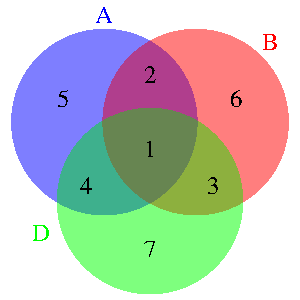
\includegraphics{InfBayes_files/figure-latex/Venn-1.pdf}

\begin{enumerate}
\def\labelenumi{(\roman{enumi})}
\tightlist
\item
  \((1) \cup (2) \cup (4) \cup (5) \precsim (1) \cup (2) \cup (3) \cup (6)\) \(~\Rightarrow~ (4) \cup (5) \precsim (3) \cup (6)\).\\
\item
  Analogamente, \((2) \cup (6) \precsim (4) \cup (7)\)
\end{enumerate}

De (i) e (ii) e pelo Lema 1, \((4) \cup (5) \cup (2) \cup (6) \precsim (3) \cup (6) \cup (4) \cup (7)\)
\(~\Rightarrow~ (2) \cup (5) \precsim (3) \cup (7)\) \(~\Rightarrow~ (2) \cup (5) \cup (1) \cup(4) \precsim (3) \cup (7) \cup (1) \cup(4)\).

\begin{center}\rule{0.5\linewidth}{0.5pt}\end{center}

\(~\)

\textbf{Teorema 2 (generalização do SP2):}
Se \(A_1, \ldots, A_n\) são eventos disjuntos e \(B_1, \ldots, B_n\) são também eventos disjuntos tais que \(A_i \precsim B_i\), para \(i=1,\ldots,n\), então \[\bigcup_{i=1}^{n} A_i \precsim \bigcup_{i=1}^{n} B_i.\]
Se \(A_i \prec B_i\) para algum i, então \(\bigcup_{i=1}^{n} A_i \prec \bigcup_{i=1}^{n} B_i.\)

\begin{center}\rule{0.5\linewidth}{0.5pt}\end{center}

\textbf{Demo:} Exercício.

\begin{center}\rule{0.5\linewidth}{0.5pt}\end{center}

\(~\)

\textbf{Teorema 3:}
Se \(A \precsim B\) então \(A^c \succsim B^c\).

\begin{center}\rule{0.5\linewidth}{0.5pt}\end{center}

\textbf{Demo:} Do Lema 1, \(A \cup (A^c \cap B^c) \precsim B \cup (A^c \cap B^c)\) \(\Rightarrow B^c \cup (A \cap B) \precsim A^c \cup (A \cap B)\) \(\Rightarrow B^c \precsim A^c\).

\begin{center}\rule{0.5\linewidth}{0.5pt}\end{center}

\(~\)

\textbf{Resultado:} Para todo evento \(A\), \(A \precsim \Omega\).

\begin{center}\rule{0.5\linewidth}{0.5pt}\end{center}

\textbf{Demo:} Por SP3, \(\emptyset \precsim A^c\). Tomando \(D=A\) no Lema 1, \(\emptyset \cup A \precsim A^c \cup A \Rightarrow A \precsim \Omega\).

\begin{center}\rule{0.5\linewidth}{0.5pt}\end{center}

\(~\)

\textbf{Teorema 4:}
Se \(A \subseteq B\) então \(A \precsim B\).

\begin{center}\rule{0.5\linewidth}{0.5pt}\end{center}

\textbf{Demo:} Suponha, \(B \prec A\). Tomando \(D=B^c\) no Lema 1, \(B \cup B^c \prec A \cup B^c \Rightarrow \Omega \prec A \cup B^c\). Absurdo!

\begin{center}\rule{0.5\linewidth}{0.5pt}\end{center}

\(~\)

\begin{center}\rule{0.5\linewidth}{0.5pt}\end{center}

\textbf{Exemplo 1:} \(\omega_0 \in \Omega\). \(A \precsim B \Leftrightarrow \{\omega_0 \in B\) \textbf{ou} \(\omega_0 \notin (A \cup B)\}\). Mostre que \(\precsim\) obedece a SP1 a SP4.

(SP1)

\(A \precsim B \Leftrightarrow \omega_0 \in B \cup (A \cup B)^c\)
\(\Rightarrow B \prec A \Leftrightarrow \omega_0 \in B^c \cap (A \cup B)\)
\(\Leftrightarrow \omega_0 \in A \cap B^c.\)

Analogamente, \(A \prec B \Leftrightarrow \omega_0 \in B \cap A^c.\)

\(A \sim B \Leftrightarrow A \precsim B\) e \(B \precsim A\)
\(\Leftrightarrow \omega_0 \in [B \cup (A \cup B)^c] \cap [A \cup (A \cup B)^c]\)
\(\Leftrightarrow \omega_0 \in (A \cap B) \cup (A \cup B)^c.\)

(SP2)

\(A_i \precsim B_i , i=1,2 \Leftrightarrow\) \(\omega_0 \in [B_1 \cup (A_1 \cup B_1)^c] \cap [B_2 \cup (A_2 \cup B_2)^c]\) \(\Leftrightarrow \omega_0 \in [(B_1 \cup B_2) \cap D^c] \cup (A_1 \cup B_1 \cup A_2 \cup B_2)^c,\)

com \(D = (A_1 \cap B2) \cup (A_2 \cap B1).\)

\(A_1 \cup A_2 \precsim B_1 \cup B_2 \Leftrightarrow\) \(\omega_0 \in (B_1 \cup B_2) \cup (A_1 \cup A_2 \cup B_1 \cup B_2)^c\)

Como \((B_1 \cup B_2) \cap D^c \subseteq (B_1 \cup B_2)\), vale o SP2.

(SP3)

\(\emptyset \precsim A \Leftrightarrow \omega_0 \in A \cup (\emptyset \cup A)^c\) \(\Leftrightarrow \omega_0 \in A \cup A^c = \Omega.\)

Como \(\Omega\) é não-vazio, \(\exists \omega_0 \in \Omega\) e, portanto, \(\emptyset \prec \Omega\).

(SP4) Exercício!

\begin{center}\rule{0.5\linewidth}{0.5pt}\end{center}

\begin{center}\rule{0.5\linewidth}{0.5pt}\end{center}

\textbf{Exemplo 2:} \(\Omega = \mathbb{N}\), \(\mathcal{A} = \mathcal{P}(\mathbb{N})\). \(A \precsim B \Leftrightarrow \{B\) é infinito \textbf{ou} \(A\) e \(B\) são finitos com \(|A| \leq |B|\}\). Verifique se \(\precsim\) satisfaz SP1 a SP4.

\begin{center}\rule{0.5\linewidth}{0.5pt}\end{center}

\(~\)

\textbf{Teorema 5:} Se \(A_1 \subseteq A_2 \subseteq \ldots\) é uma sequência crescente de eventos e \(B\) é tal que \(A_n \precsim B, \forall n\) então \[\bigcup_{n \geq 1} A_n \precsim B.\]

\begin{center}\rule{0.5\linewidth}{0.5pt}\end{center}

\textbf{Demo:} \(A_n^c \supseteq A_{n+1}^c\) e, pelo Teo 3, \(A_n^c \succsim B^c\), \(\forall n\).

Por SP4, \(\bigcap_{n \geq 1} A_n^c \succsim B^c\) \(\Rightarrow \bigcup_{n \geq 1} A_n \precsim B.\)

\begin{center}\rule{0.5\linewidth}{0.5pt}\end{center}

\(~\)

\textbf{Teorema 6:} \(\left(A_n\right)_{n \geq 1}\) e \(\left(B_n\right)_{n \geq 1}\) sequências tais que \(A_i \cap A_j = B_k \cap B_l = \emptyset\), \(\forall i \neq j\), \(\forall k \neq l\).
\[A_i \precsim B_i, \forall i ~\Rightarrow~ \bigcup_{n \geq 1} A_n \precsim \bigcup_{n \geq 1} B_n.\]
Se existe ao menos um \(j\) tal que \(A_j \prec B_j\) então \(\displaystyle{ \bigcup_{n \geq 1} A_n \prec \bigcup_{n \geq 1} B_n }.\)

\begin{center}\rule{0.5\linewidth}{0.5pt}\end{center}

\textbf{Demo:} Da extensão de SP2, temos que \(\displaystyle{ \bigcup_{i = 1}^n A_i \precsim \bigcup_{i = 1}^n B_i }\), \(\forall n \geq 1\) \(~\Rightarrow~ \displaystyle{ \bigcup_{i = 1}^n A_i \precsim \bigcup_{i = 1}^{\infty} B_i }\), \(\forall n \geq 1\) \(~\Rightarrow~ \displaystyle{ \bigcup_{i = 1}^{\infty} A_i \precsim \bigcup_{i = 1}^{\infty} B_i }~\) (Teo 5)

\(\exists n_0\) tal que \(A_{n_0} \prec B_{n_0}\). De SP2, temos que, para \(n \geq n_0\),

\(\displaystyle \bigcup_{i = 1}^{n_0} A_i = \bigcup_{i = 1}^{n_0-1} A_i \cup A_{n_0} \prec \bigcup_{i = 1}^{n_0-1} B_i \cup B_{n_0} = \bigcup_{i = 1}^{n_0} B_i\) \(~\Rightarrow~ \displaystyle \bigcup_{i = 1}^{n_0} A_i \prec \bigcup_{i = 1}^{n_0} B_i.\)

Da primeira parte, temos que \(\displaystyle{ \bigcup_{i = n_0+1}^{\infty} A_i \precsim \bigcup_{i = n_0+1}^{\infty} B_i } ~\) e, por SP2,

\(\displaystyle \bigcup_{i = 1}^{n_0} A_i \cup \bigcup_{i = n_0+1}^{\infty} A_i \prec \bigcup_{i = 1}^{n_0} B_i \cup \bigcup_{i = n_0+1}^{\infty} B_i\)

provando o resultado.

\begin{center}\rule{0.5\linewidth}{0.5pt}\end{center}

\(~\)

\hypertarget{aula-03}{%
\section{Aula 03}\label{aula-03}}

\hypertarget{medida-de-probabilidade-que-representa-precsim}{%
\subsection{\texorpdfstring{Medida de Probabilidade que ``representa'' \(\precsim\)}{Medida de Probabilidade que ``representa'' \textbackslash precsim}}\label{medida-de-probabilidade-que-representa-precsim}}

\textbf{Teorema 7:} Seja \(A \in \mathcal{A}\). Então \(\exists! a^* \in [0,1]\) tal que \(A \sim \{X \in [0,a^*]\}\).

\begin{center}\rule{0.5\linewidth}{0.5pt}\end{center}

\textbf{Demo:} Seja \(U(A) = \left\{ a \in [0,1] : A \precsim \{X \in [0,a]\} \right\}\).

\(1 \in U(A)\) pois \(\Omega = \{X \in [0,1]\} \succsim A\) \(~\Rightarrow~ U(A) \neq \emptyset\).

Tome \(a^* = \inf U(A)\).

\begin{enumerate}
\def\labelenumi{(\roman{enumi})}
\item
  Considere \((a_n)_{n \geq 1}\), \(a_n \in [0,1], \forall n \geq 1\), tal que \(a_n \geq a_{n+1} \geq a^*\) e \(a_n \downarrow a^*\). Então, \(\forall n \geq 1\) , \(\{X \in [0,a_n]\} \succsim A\).\\
  Por SP4, \(\displaystyle \bigcap_{n=1}^\infty \{X \in [0,a_n]\} \succsim A\) \(~\Rightarrow~ \{X \in [0,a^*]\} \succsim A\)
\item
  Se \(a^*=0\) , \(\{X \in [0,0]\} \sim \emptyset \precsim A\) (por SP3).\\
  Se \(a^* > 0\) , considere \((a_n)_{n \geq 1}\) com \(a_n \leq a_{n+1} < a^*\) e \(a_n \uparrow a^*\).\\
  \(\{X \in [0,a_n]\} \precsim A, \forall n \geq 1\) e, pelo Teo 5, \(\displaystyle \bigcup_{n=1}^{\infty} \{X \in [0,a_n]\} \precsim A\) \(~\Rightarrow~ \{X \in [0,a^*)\} \sim \{X \in [0,a^*]\} \precsim A\).
\end{enumerate}

De (i) e (ii), temos que \(A \sim \{X \in [0,a^*]\}\).

\(a^*\) é único pois se \(a_1 < a^* < a_2\) são outros valores quaisquer, segue que \(\{X \in [0,a_1]\} \prec \{X \in [0,a^*]\} \prec \{X \in [0,a_2]\}\) e só um desses eventos pode ser equivalente à \(A\).

\begin{center}\rule{0.5\linewidth}{0.5pt}\end{center}

\(~\)

\textbf{Teorema 8:} A probabilidade do evento \(A\), \(P(A)\), é definida como \(a^* \in [0,1]\) tal que \(A \sim \{X \in [0,a^*]\}\). Assim, \(A \sim \left\{X \in \left[0,P(A)\right]\right\}\). A função de probabilidade assim definida satisfaz:
\[A \precsim B ~\Leftrightarrow~ P(A) \leq P(B).\]

\begin{center}\rule{0.5\linewidth}{0.5pt}\end{center}

\textbf{Demo:} Do Teo 7, \(A \sim \left\{X \in \left[0,P(A)\right]\right\}\) e \(B \sim \left\{X \in \left[0,P(B)\right]\right\}\).

\(A \precsim B\) \(~\Leftrightarrow~ \left\{X \in \left[0,P(A)\right]\right\} \precsim \left\{X \in \left[0,P(B)\right]\right\}\) \(~\Leftrightarrow~ \lambda \left([0,P(A)]\right) \precsim \lambda \left([0,P(B)]\right)\) \(~\Leftrightarrow~ P(A) \leq P(B).\)

\begin{center}\rule{0.5\linewidth}{0.5pt}\end{center}

\(~\)

\textbf{Teorema 9:} A função \(P: \mathcal{A} \longrightarrow [0,1]\) que, para cada \(A \in \mathcal{A}\), associa \(P(A)\) tal que \(A \sim \left\{X \in \left[0,P(A)\right]\right\}\) é uma medida de probabilidade (no sentido \(\sigma\)-aditiva).

\begin{center}\rule{0.5\linewidth}{0.5pt}\end{center}

\textbf{Demo:}

\begin{enumerate}
\def\labelenumi{(\roman{enumi})}
\item
  \(P(A) \geq 0\).\\
  \(\Omega \sim \{X \in [0,1]\}\Rightarrow P(\Omega)=1\).\\
  \(\emptyset \sim \{X \in [0,0]\} \Rightarrow P(\emptyset)=0\)\\
  \(\emptyset \precsim A \Rightarrow 0 \leq P(A)\).
\item
  Seja \(A\) e \(B\) tal que \(A \cap B = \emptyset\). Vamos mostrar que \(P(A \cup B) = P(A) + P(B)\).\\
  Pelo Teo 8, \(A \sim \{ X \in [0,P(A)]\}\), \(B \sim \{ X \in [0,P(B)]\}\), \(A \cup B \sim \{ X \in [0,P(A \cup B)]\}\).\\
  Como \(A \subseteq A \cup B\) e, por SP3, \(A \precsim A \cup B\), vale que \(P(A) \leq P(A \cup B)\). Vamos verificar que \(B \sim \left\{X \in \left(P(A),P(A \cup B) \right]\right\}\).\\
  Suponha, por absurdo, \(B \prec \left\{X \in \left(P(A),P(A \cup B) \right]\right\}\).\\
  \(A \precsim \{X \in [0,P(A)]\}\) \(~\overset{SP2}{\Longrightarrow}~\)
  \(A \cup B \prec \{X \in [0,P(A)]\} \cup \left\{X \in \left(P(A),P(A \cup B) \right]\right\}\)
  \(~\Rightarrow~ A \cup B \prec \left\{X \in [0,P(A)] \cup \left(P(A),P(A \cup B) \right]\right\}\)
  \(~\Rightarrow~ A \cup B \prec \left\{X \in \left[0,P(A \cup B) \right]\right\}\) \textasciitilde{} (Absurdo!)\\
  Analogamente, \(B \succ \left\{X \in \left(P(A),P(A \cup B) \right]\right\}\) é absurdo! Logo, \(B \sim \left\{X \in \left(P(A),P(A \cup B) \right]\right\} \sim \left\{X \in \left[0, P(A \cup B)-P(A) \right]\right\}\).\\
  Como \(B \sim \left\{X \in \left[0,P(B)\right]\right\}\), temos que \(P(A \cup B) = P(A) + P(B)\).
\end{enumerate}

\begin{center}\rule{0.5\linewidth}{0.5pt}\end{center}

\(~\)

\textbf{Corolário 1:} Se \(A_1, \ldots, A_n\) são eventos disjuntos, então \(P\left(\bigcup_{i=1}^{n} A_i\right) = \sum_{i=1}^{n} P\left(A_i\right)\).

\begin{center}\rule{0.5\linewidth}{0.5pt}\end{center}

\textbf{Demo:} Indução.

\begin{center}\rule{0.5\linewidth}{0.5pt}\end{center}

\(~\)

\textbf{Teorema 10:} Seja \(A_1 \supseteq A_2 \supseteq \ldots\) uma seq. decrescente de eventos tais que \(\bigcap_{i=1}^{n} A_i = \emptyset\). Então \(\displaystyle \lim_{n \uparrow \infty} P(A_n) = 0\).

\begin{center}\rule{0.5\linewidth}{0.5pt}\end{center}

\textbf{Demo:} \(A_1 \supseteq A_2 \supseteq \ldots\) \(\Rightarrow\) \(P(A_1) \geq P(A)_2 \geq \ldots\).

Além disso, \(\displaystyle \lim_{n \uparrow \infty} P(A_n) = b\). Como \(P(A_n) \geq b\), \(\forall n\), segue que \(A_n \succsim \{X \in [0,b]\}\), \(\forall n\).

Por SP4, \(\emptyset = \bigcap_{i=n}^{\infty} A_i \succsim \{X \in [0,b]\}\).

Se \(b>0\), então \(\{X \in [0,b]\} \succ \{X \in [0,b/2]\} \succsim \emptyset\). Como essa relação contradiz a anterior, temos que \(b\) deve ser igual a \(0\).

\begin{center}\rule{0.5\linewidth}{0.5pt}\end{center}

\(~\)

\textbf{Exercício 1:}
Use o Corolário 1 e o Teorema 10 para conculuir a demonstração do Teorema 9, mostrando que \(P\) é \(\sigma\)-aditiva, isto é, \[P\left(\bigcup_{i=1}^{\infty} A_i\right) = \sum_{i=1}^{\infty} P\left(A_i\right) ~,~~ A_i \cap A_j = \emptyset, \forall i \neq j.\]

\begin{center}\rule{0.5\linewidth}{0.5pt}\end{center}

\textbf{Solução:} Seja \((A_n)_{n \geq 1}\) sequência de eventos disjuntos. Segue do Corolário 1 que\\
(i) \(\displaystyle P\left(\bigcup_{i=1}^{\infty} A_n\right) = \sum_{i=1}^{n} P\left(A_i\right) + P\left(\bigcup_{j=n+1}^{\infty} A_j\right)\), \(n=1,2,\ldots\)

Considere \(\displaystyle B_n=\bigcup_{j=n+1}^{\infty} A_j\), \(n \geq 1\), uma sequência decrescente de eventos tais que \(\displaystyle \bigcap_{n=1}^{\infty} B_n = \emptyset\). Pelo Teorema 10, segue que \(\displaystyle \lim_{n\uparrow \infty} B_n = 0\). Assim, tomando o limite do lado direito de (i), segue que

\(\displaystyle P\left(\bigcup_{i=1}^{\infty} A_n\right)\) \(=\displaystyle \lim_{n\uparrow \infty} \sum_{i=1}^{n} P\left(A_i\right) + \lim_{n\uparrow \infty} P\left(B_n\right)\) \(=\displaystyle \sum_{i=1}^{\infty} P\left(A_i\right)\).

\begin{center}\rule{0.5\linewidth}{0.5pt}\end{center}

\(~\)

\textbf{Teorema 11:} Se a relação de crença \(\precsim\) obedece SP1 a SP5 então \(\exists !~ P: \mathcal{A} \rightarrow [0,1]\), medida de probabilidade, tal que \(P\) representa \(\precsim\).

\begin{center}\rule{0.5\linewidth}{0.5pt}\end{center}

\textbf{Demo:} Exercício!

\begin{center}\rule{0.5\linewidth}{0.5pt}\end{center}

\(~\)

\hypertarget{medida-de-probabilidade-condicional}{%
\subsection{Medida de Probabilidade Condicional}\label{medida-de-probabilidade-condicional}}

\textbf{Nova Relação:} \((A|D) \precsim (B|D)\) (Sabendo que \(D\) ocorreu, \(B\) é preferível a \(A\)).

\begin{itemize}
\item
  Para \(D = \Omega\), temos o caso anterior: \(A \precsim B\) \(\Leftrightarrow (A|\Omega) \precsim (B|\Omega)\).
\item
  Suponha que vale as suposições SP1 a SP5 e, adicionalmente,
\end{itemize}

\begin{quote}
SP6: \((A|D) \precsim (B|D) \Leftrightarrow (A \cap D) \precsim (B \cap D)\) \(~~\Big( (A \cap D|\Omega) \precsim (B \cap D|\Omega) \Big)\)
\end{quote}

\textbf{Teorema 12:} \(\forall A, B, D \in \mathcal{A}\), considere \(\precsim\) satisfazendo SP1 a SP6. Então \(P: \mathcal{A} \rightarrow [0,1]\) de modo que para cada \(A \in \mathcal{A}\) é associada \(P(A) \in [0,1]\) tal que \(A \sim \left\{X \in \left[0,P(A)\right]\right\}\) é uma medida de probabilidade que representa \(\precsim\), isto é, \[(A|\Omega) \precsim (B|\Omega) \Leftrightarrow P(A) \leq P(B).\] Além disso, se \(D \in \mathcal{A}\) é tal que \(P(D) \geq 0\), então \[(A|D) \precsim (B|D) \Leftrightarrow P(A|D) \leq P(B|D),\] onde \(P(\cdot|D): \mathcal{A} \rightarrow [0,1]\) é uma medida de probabilidade tal que
\[P(A|D) = \frac{P(A \cap D)}{P(D)}.\]

\hypertarget{literature}{%
\chapter{Literature}\label{literature}}

Here is a review of existing methods.

\hypertarget{methods}{%
\chapter{Methods}\label{methods}}

We describe our methods in this chapter.

\hypertarget{applications}{%
\chapter{Applications}\label{applications}}

Some \emph{significant} applications are demonstrated in this chapter.

\hypertarget{example-one}{%
\section{Example one}\label{example-one}}

\hypertarget{example-two}{%
\section{Example two}\label{example-two}}

\hypertarget{final-words}{%
\chapter{Final Words}\label{final-words}}

We have finished a nice book.

  \bibliography{bibliografia.bib,packages.bib}

\end{document}
